\documentclass{standalone}

\usepackage{tikz}
\usepackage{circuitikz}

\tikzset{block/.style = {draw, fill=white, very thick, rectangle, minimum height=1cm, minimum width=2cm},
         lblock/.style={draw,fill=white,very thick, rectangle, minimum height=3cm, minimum width=1cm},
         sum/.style= {draw, fill=white, very thick, circle, node distance=0.5cm}}

         
\begin{document}
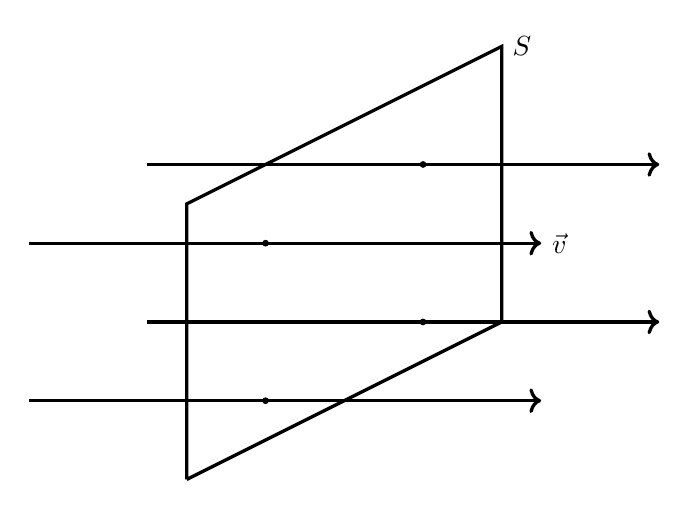
\begin{tikzpicture}[scale=2]
    \draw[very thick](0,0)--(0,1.75)--(2,2.75)node[right]{$S$}--(2,1)--(0,0);
    
    \draw[->,very thick](-1,0.5)--(2.25,0.5);
    \draw[->,very thick](-0.25,1)--(3,1);
    \draw[->,very thick](-1,1.5)--(2.25,1.5)node[right]{$\vec{v}$};
    \draw[->,very thick](-0.25,2)--(3,2);

    \filldraw[black](0.5,0.5)circle(0.5pt);
    \filldraw[black](1.5,1)circle(0.5pt);
    \filldraw[black](0.5,1.5)circle(0.5pt);
    \filldraw[black](1.5,2)circle(0.5pt);
\end{tikzpicture}
\end{document}